\section{Introduction}
\label{sec:intro}

\todoRevise{review introduction}

Being able to reconstruct shapes from partial representations is a useful tool in medical applications.
For example, one could be interested in the original shape of remaining parts of a bone fracture, which enables building suitable artificial implants.
Many more similar fields of applications could be imagined.
However, in this paper we only consider the specific problem of reconstructing femur bones from partial femur shapes as depicted in \autoref{fig:partial}.
\begin{figure}[b]
	\centering
  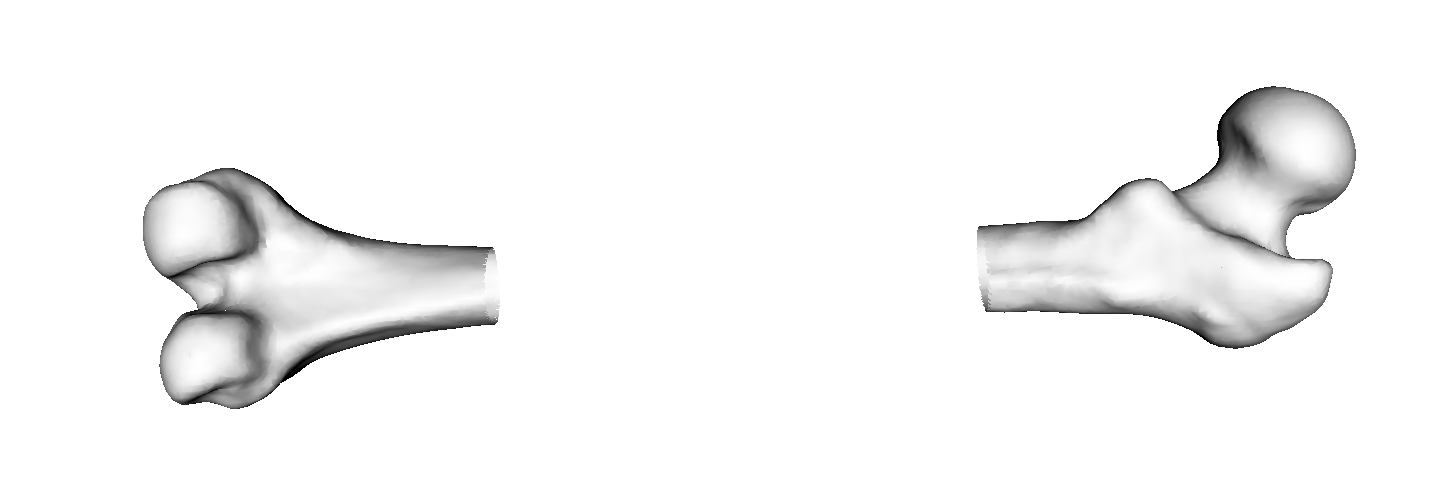
\includegraphics[scale=.15]{./Figures/partial_femur}
  \caption{Incomplete data of a femur bone.}
  \label{fig:partial}
\end{figure}

Knowing typical characteristics of the underlying shape is essential, in order to estimate a high-quality reconstruction.
It can be learned from complete data of the corresponding shape families.
We call the result of this learning process a \emph{statistical shape model}.

This paper reports our findings from the project posed in the Future Learn course called ``Statistical Shape Modelling: Computing the Human Anatomy''~\cite{mooc2019statistical}.
The most part of the theory used is also acquired from that course.
